\section{Evaluation}
\label{sec:evaluation}

To evaluate \name, we integrated our end-to-end prototype in \company, and ran a pilot deployment across the above network to serve 70 TB data per day per hour  over a period of 7 days.
The evaluation results of the pilot deployment, together with trace-driven simulation and microbenchmarks, show that:
\begin{packedenumerate}
\item \name completes bulk-data multicast 3-5$\times$ faster than \company's existing solution, as well as other industry-standard solutions (\Section\ref{subsec:evaluation:centralized}).
\item \name eliminates interference with latency-sensitive data using a clean bandwidth separation (\Section\ref{subsec:evaluation:separation}).
\item \name can update decisions over a WAN of the same size as B4, while still being lightweight in terms of CPU, bandwidth consumed (\Section\ref{subsec:evaluation:benchmarks}).
\end{packedenumerate}

\begin{figure*}[t]
        \centering
        \begin{subfigure}[b]{0.3\textwidth}
                \centering
                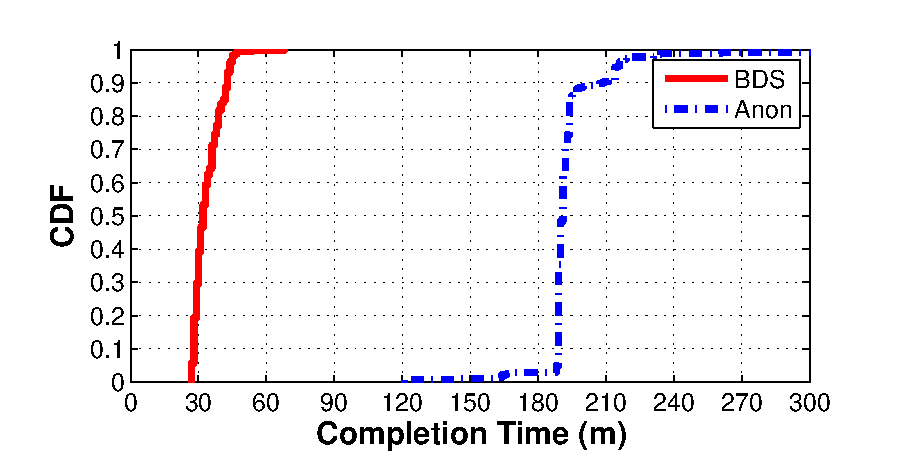
\includegraphics[width=\textwidth]{images/BDSvsAnon_overall.eps}
                \caption{The completion time.}
                \label{fig:BDSvsAnon:overall}
        \end{subfigure}
        \begin{subfigure}[b]{0.3\textwidth}%@X:\6 PieBridge\simulation\beijing\3 Applications\plot
                \centering
                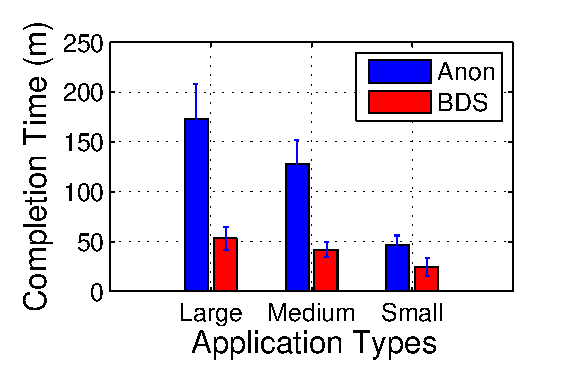
\includegraphics[width=\textwidth]{images/BDS_VS_ANON_v3.eps}
                \caption{Comparison by application types.}
                \label{fig:BDSvsAnon:FCT}
        \end{subfigure}
        \begin{subfigure}[b]{0.3\textwidth}
                \centering
                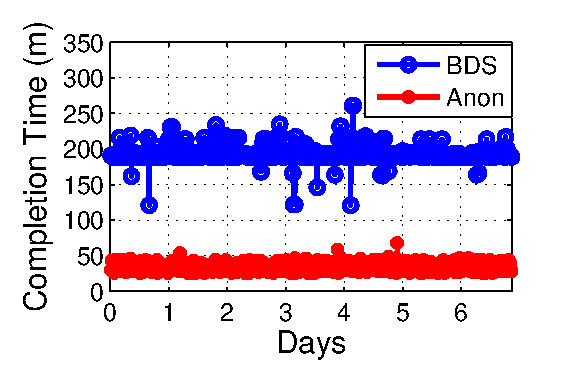
\includegraphics[width=\textwidth]{images/BDSvsAnon_time.eps}
                \caption{Comparison by timeseris.}
                \label{fig:BDSvsAnon:time}
        \end{subfigure}
        \caption{[\name vs. \company] Results from pilot deployments.}
        \label{fig:BDSvsAnon}
\vspace{-0.4cm}
\end{figure*}
%\begin{figure*}[t] %@X:\6 PieBridge\simulation\DrawFig
%        \centering
%        \begin{subfigure}[b]{0.3\textwidth}
%                \centering
%                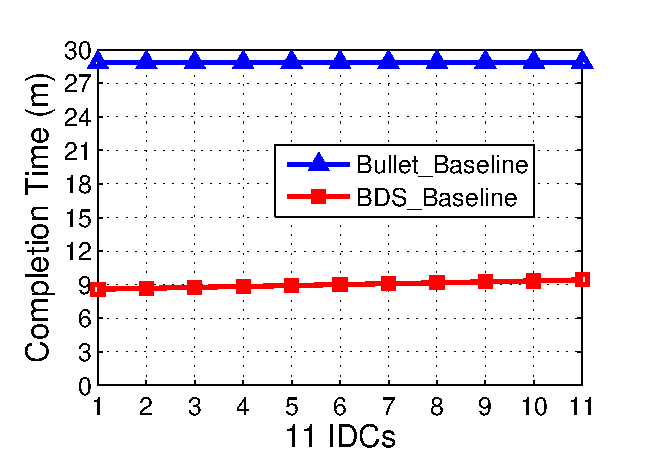
\includegraphics[width=50mm]{images/Test1.eps}
%                \caption{Baseline experiment.}
%                \label{fig:cdn:baseline}
%        \end{subfigure}
%        \begin{subfigure}[b]{0.3\textwidth}
%                \centering
%                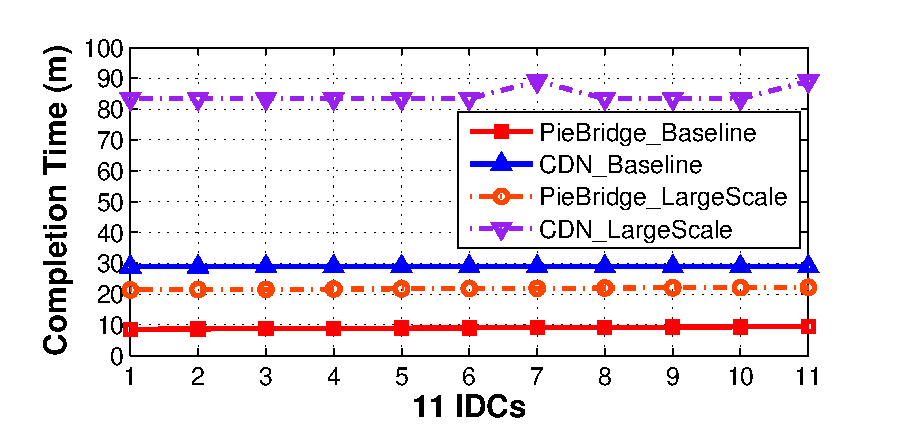
\includegraphics[width=50mm]{images/Test2.eps}
%                \caption{Large scale experiments.}
%                \label{fig:cdn:scale}
%        \end{subfigure}
%        \begin{subfigure}[b]{0.3\textwidth}
%                \centering
%                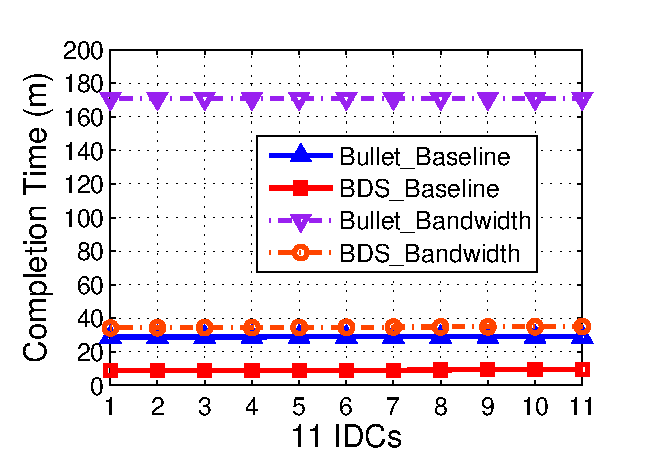
\includegraphics[width=50mm]{images/Test3.eps}
%                \caption{Small bandwidth experiments.}
%                \label{fig:cdn:bw}
%        \end{subfigure}
%        \caption{[\name versus Bullet] Comparisons under different network scenarios.}
%        \label{fig:versusCDN}
%\vspace{-0.4cm}
%\end{figure*}


\subsection{Benefits of centralized control}
\label{subsec:evaluation:centralized}

We compare \name's against three baselines in terms of
multicast completion time:
\company's existing solution (a decentralized strategy),
Bullet~\cite{kostic2003bullet} (a centralized strategy), and
Akamai's overlay network~\cite{Andreev2013Designing} for live video streaming
multicast.

\tightsubsubsection{Methodology}

Pilot deployment. We choose a service with 70~TB daily data file to transfer. In general, this bulk data is transferred by \company's existing solution (that has already run for more than 5 years), while we randomly choose several days using \name instead of the current solution. To make sure the two solutions work in the same environment, we conduct the following experiments at the same time of a day.

Trace-driven simulation. For safety reasons, we cannot implement other solutions on the real network, so we simulate the other two overlay multicast techniques and evaluate their performance using real data trace. We set the same topology, source DC, destination DCs, server configurations as the real environments, and compare the results against \name.


%To evaluate the benefits of centralized control, we conduct two series of experiments: the comparisons with \company's existing solution based on the pilot deployments, and the comparisons with other overlay multicast techniques using trace-driven simulations.

\tightsubsubsection{\name vs. \company's existing solution}

The above mentioned 70~TB data file is distributed stored in the source DC (with 1000 servers) at the very beginning, and each of the other DCs announces a downloading requirement and finally stores the file in the same way with 1000 servers.

%First of all, we present the completion time of destination servers under \name and \company in Figure

To intuitively present the overall improvements by \name, we draw the CDF of the completion time in Figure \ref{fig:BDSvsAnon:overall}, from which we can see that the completion time under \company's existing solution is about 200 minutes while that of \name is less than 40 minutes, 5 times shorter completion time.

For detailed illustration, we pick three applications whose data volumes are large, medium and small, and draw a bar chart of three pairs of bars in Figure \ref{fig:BDSvsAnon:FCT}, each representing \name's and \company's mean (stddev) completion time for one application. These bars show that for small data volume, \name outperforms 1.6$\times$ than \company, but raises up to more than 3$\times$ than \company for large data volume. In other words, the benefit of \name will increase along with the data volumes.

To prove that this is not a special case, we repeat the experiments during the 7 days, and draw the average completion time of both \name and \company in Figure \ref{fig:BDSvsAnon:time}. \name is quite stable during the 7 days while \company illustrates some volatilities. But in general, \name achieves about 4.5$\times$ shorter completion time than \company.
%\item \name vs. \company's existing solution (pilot deployment)
%\begin{itemize}
%\item Overall improvement: A CDF with two lines to show the aggregated flow completion time
%\item By applications: Pick three applications whose data volumes are large, medium, and small respectively. Draw a bar chart of three pairs of bars, each representing \name's and \company's mean (stddev) flow completion time for an application.
%\item By time: Timeseris of two lines, each representing \name's and \company's mean (stddev) of flow completion time.
%\end{itemize}

\tightsubsubsection{\name vs. other overlay multicast techniques}

%As we cannot implement other experimental systems in our real online network just as comparisons, we conduct a series of simulations using trace-driven simulations in this section, and compare \name's performance versus Bullet \cite{kostic2003bullet} and a CDN-based solution \cite{Andreev2013Designing} adopted by Akamai.

We use the same topology with 12 DCs (1 DC acts as the source DC) for all simulations, and set the parameters all the same as the real network, including data file size, data source and destination, paths, link capacities and server upload/download rates.

Bullet \cite{kostic2003bullet} is a distributed algorithm that works on an overlay mesh network, it enables geo-spread nodes to self-organize into a overlay mesh. Specifically, each node uses RanSub \cite{Rodriguez2003Using} to distribute summary tickets information to other nodes, and receives disjoint data from his sending peers. The most obvious difference between \name and Bullet lies in the control scheme, i.e., \name is centralized method, who can maximize total system traffic, while Bullet is a decentralized scheme and each node makes decision according to his obtained information.

Akamai design a 3-layer overlay network for delivering live streams \cite{Andreev2013Designing}, where a source forwards its streams to reflectors, and a reflector sends outgoing streams to the final stage sinks. Things \name and Akamai have in common is that both of them are designed for data distribution on overlay multicast networks. There are two main differences  between Akamai and \name: (1) Akamai adopts a 3-layer topology where an edgeserver receives data from the parent reflectors, while \name could explore more potential searching space without layer limitation. (2) A sink in Akamai receives must receive data in sequential order because it serves for the live streaming application, but \name does care about blocks arriving order. Thus, to achieve optimal scheduling results, \name should also solve the scheduling problem so as to work out the optimal block download order $\overrightarrow{o}(s_i)$.

%We conduct three series of experiments and show the results in Figure \ref{fig:versusCDN}: baseline \ref{fig:cdn:baseline}, large scale \ref{fig:cdn:scale} and small bandwidth experiments \ref{fig:cdn:bw}. We find \name achieves 3$\times$ shorter completion time than Bullet in the baseline experiments, and more than 4$\times$ improvement in the large scale experiments and small bandwidth experiments.
We conduct three series of experiments and show the results in Table \ref{table:versusAkamai}: baseline, large scale and small bandwidth experiments. In the baseline experiments, the size of the bulk data is 10TB , the number of server per DC is 100, and the upload/download rate limits are set to 20Mbps, while in the large scale experiment, the bulk data is 100TB, server number per DC is 1000, and in the small bandwidth experiment, server upload/download rate limit is reduced to 5M/bps. We find that \name achieves 3$\times$ shorter completion time than Bullet and Akamai in the baseline experiments, and more than 4$\times$ improvement in the large scale experiments and small bandwidth experiments.

In the large scale experiments, the completion time of Bullet increases to about 3 times than that in the baseline experiment, and that of Akamai multicast solution is about 3.5 times. But \name only increase to about 2 times. This advantage proves \name's good scalability. In the small bandwidth experiments (when delay-sensitive traffic bursts, such bandwidth reduction is very common), the completion time of \name increase to about 4 times while that of Bullet and Akamai is 6.1 and 5.52, respectively. These results illustrate the high transmission efficiency of \name.

\begin{table}[t]
\begin{center}
\resizebox{3in}{!}{
%\begin{tabular}{p{2cm}<{\centering}|p{2cm}<{\centering}}
\begin{tabular}{| c | c| c| c|}
\hline
 \rowcolor[gray]{0.9}
\textbf{Solution} & \textbf{Baseline} & \textbf{Large Scale} & \textbf{Rate Limit} \\
\hline \hline
Bullet & $28m$ & $82m$ & $171m$\\
\hline
Akamai & $25m$ & $87m$ & $138m$\\
\hline
\name & $9.41m$ & $20.33m$ & $38.25m$\\
\hline
\end{tabular}
}
\end{center}
\vspace{-0.4cm}
\caption{[\name vs. Bullet \cite{kostic2003bullet}, Akamai \cite{Andreev2013Designing}] Results from trace-driven simulations.}
%\caption{Average completion time of Bullet \cite{kostic2003bullet}, Akamai \cite{Andreev2013Designing} and \name.}
\label{table:versusAkamai}
\end{table}

%\begin{itemize}
%\item \name vs. other overlay multicast techniques
%\begin{itemize}
%\item Begin with the methodology of trace-driven simulation.
%\item Briefly explain these techniques: Akamai (3-layer), Bullet (full mesh)
%\item Show a CDF that has three lines, representing \name, Akamai, and Bullet.
%\end{itemize}
%\end{itemize}

\subsection{Benefits of bandwidth separation}
\label{subsec:evaluation:separation}
\begin{figure}[t]
  \centering
  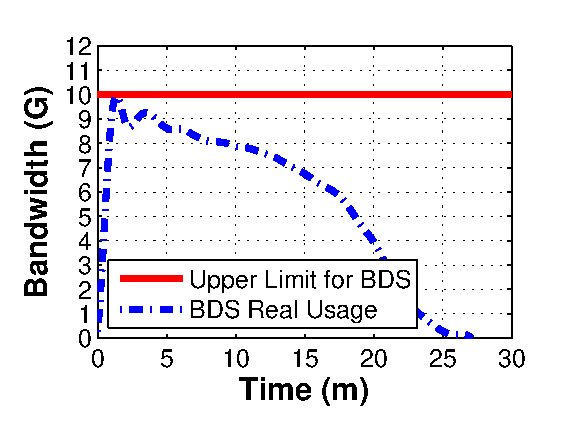
\includegraphics[width=45mm]{images/Quota.eps}
  \caption{The effectiveness of bandwidth separation.}
  \label{fig:quota}
\end{figure}
%\vspace{-0.4cm}

To test the effectiveness of bandwidth separation and check whether the bulk data transfer will reserve bandwidth for latency-sensitive traffic according to the separation quota, we set the upper bound of available bandwidth for bulk data transfer to 10~Gbps, and then monitor the real usage of one inter-DC link. The results are shown in Figure \ref{fig:quota}, from which we can see the real bandwidth usage stays below the upper bound (10~Gbps) throughout the whole transmission process, verifying that the separation does take effects on link bandwidth usage and thus can reduce the incidents of delay on latency-sensitive traffic caused by bulk data transfers.

\begin{table}[t]
\begin{center}
\resizebox{.5\textwidth}{!}{%
%\begin{tabular}{p{2cm}<{\centering}|p{2cm}<{\centering}}
\begin{tabular}{| c | c | c | c | c |}
\hline
 \rowcolor[gray]{0.9}
\textbf{System} & \textbf{Link from the source DC} & \textbf{$l_1$} & \textbf{$l_2$} & \textbf{$l_3$}\\
\hline \hline
\company & 69.82\% & 53.09\% & 57.98\% & 63.01\% \\
\hline
\name & 70.55\% & 62.46\% & 63.23\% & 64.24\% \\
\hline
\end{tabular}
}
\end{center}
\caption{Average link utilizations under \company and \name.}
\label{table:usage}
\vspace{-0.4cm}
\end{table}

\begin{figure*}[t]
        \centering
        \begin{subfigure}[b]{0.3\textwidth}
                \centering
                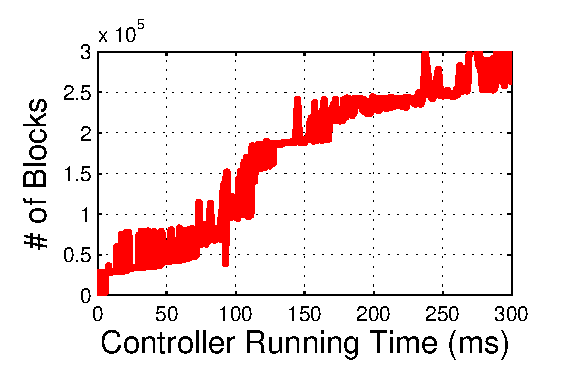
\includegraphics[width=50mm]{images/CPUvsBlk.eps}%CDFofComputationDelay -> Calculation.m
                \caption{The controller running time.}
                \label{fig:scale:cpu}
        \end{subfigure}
        \begin{subfigure}[b]{0.3\textwidth}
                \centering
                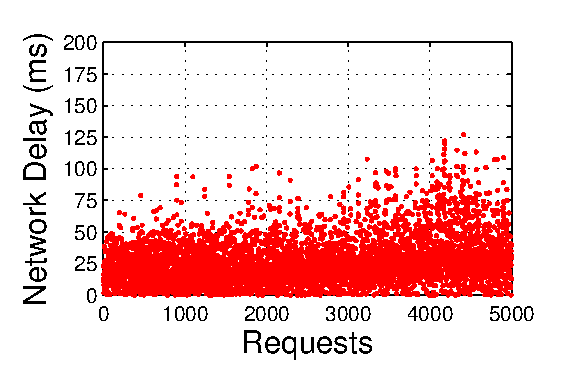
\includegraphics[width=50mm]{images/NetworkDelay.eps}%CDFofNetworkDelay -> Communication.m
                \caption{The inter-DC network delay.}
                \label{fig:scale:network}
        \end{subfigure}
        \begin{subfigure}[b]{0.3\textwidth}
                \centering
                \includegraphics[width=50mm]{images/CDFofFeedbackLoopDelay.eps}
                \caption{Feedback loop delay.}
                \label{fig:scale:feedback}
        \end{subfigure}
        \caption{[System scalability] Measurements on (a) controller running time, (b) network delay, (c) Feedback loop delay.}
        \label{fig:scale}
\vspace{-0.4cm}
\end{figure*}

\begin{figure*}[t]
        \centering
        \begin{subfigure}[b]{0.3\textwidth}
                \centering
                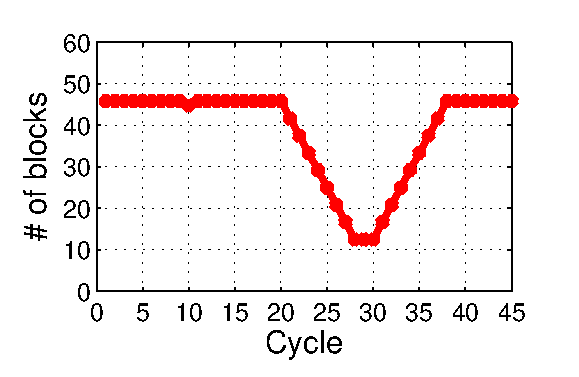
\includegraphics[width=50mm]{images/failure.eps}%fail.m
                \caption{Average number of downloaded blocks per cycle under failures.}
                \label{fig:analysis:failure}
        \end{subfigure}
        \begin{subfigure}[b]{0.3\textwidth}
                \centering
                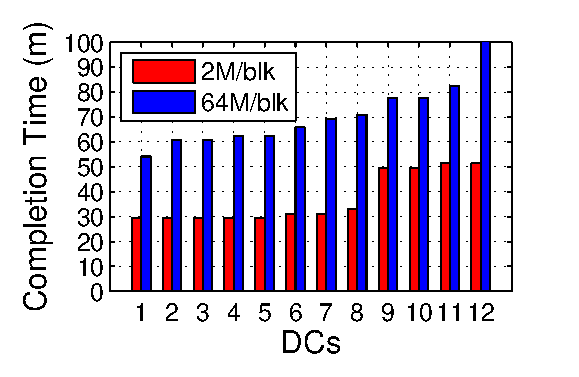
\includegraphics[width=50mm]{images/blkSize.eps} % cpu.m
                \caption{Completion time under different block sizes.}
                \label{fig:analysis:blksize}
        \end{subfigure}
        \begin{subfigure}[b]{0.3\textwidth}
                \centering
                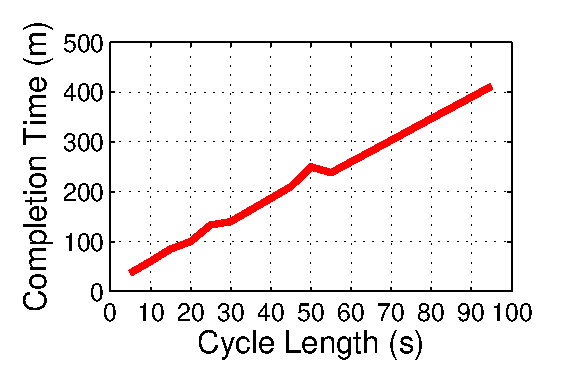
\includegraphics[width=50mm]{images/cycleDiff.eps}%cycleDiff.m
                \caption{Completion time under different cycle lengths.}
                \label{fig:analysis:cycleDiff}
        \end{subfigure}
%        \begin{subfigure}[b]{0.3\textwidth}
%                \centering
%                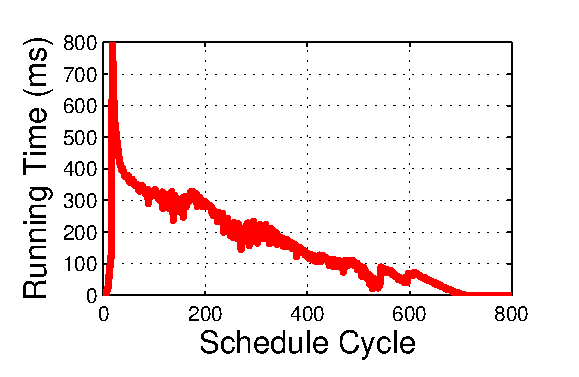
\includegraphics[width=50mm]{images/cycle.eps} %calculation_origin
%                \caption{Reduction on algorithm running time due to approximation.}
%                \label{fig:analysis:time}
%        \end{subfigure}
%        \begin{subfigure}[b]{0.3\textwidth}
%                \centering
%                \includegraphics[width=50mm]{images/overlay.eps}
%                \caption{The proportion of blocks downloaded from the original source.}
%                \label{fig:analysis:overlay}
%        \end{subfigure}
        \caption{[Algorithm adaptability] Measurements on (a) fault tolerance, (b) different block size, and (c) different cycle length.}
        \label{fig:analysis}
\vspace{-0.4cm}
\end{figure*}


As \name implements strict bandwidth separation between latency-sensitive traffic and bulk data transfer while still showing shorter completion time, does \name increase link utilization significantly? To answer this question, we record the average utilizations of: (1) the egress link of the source DC, and (2) 3 randomly selected inter-DC links, denoted as $l_1,l_2$ and $l_3$. Results are shown in Table \ref{table:usage}, which shows that link utilizations do not change much with \name or with \company. This is because \name can make disjoint data transfers to different receivers and thus avoids transferring repeated data compared the self-organized \company's solution.

%\begin{itemize}
%\item Draw a graph (what graph can you get on this?) to show with bandwidth separation, \name can reduce the incidents of delay on latency-sensitive traffic caused by bulk data transfers.%DrawLink.m
%\item Draw a graph (what graph can you get on this?) to show the link utilization does not change much with \name or with \company.%DrawUsage.m
%\end{itemize}

\subsection{Micro-benchmarks}
\label{subsec:evaluation:benchmarks}

This section focuses on some benchmarks of \name. 1. Scalability of centralized control. As \name adopts centralized control, the running time and scalability of controller are key indicators of algorithm efficiency. 2. Algorithm adaptability. \name runs on company's network, together with online latency-sensitive traffic, so high fault tolerance and strong robustness are essential requirements. 3. In-depth analysis. The benefits of \name's two approximations and the effects of exploring overlay network also need to be clarified.

\tightsubsubsection{System scalability.}

\mypara{Controller Running Time} As the controller needs to assign optimal data source, transmission path and bandwidth for all blocks, the algorithm running time is thus related to the number of blocks. We show the relationship of block number and algorithm running time in Figure \ref{fig:scale:cpu}, from which we can see that even when there are $3\times 10^5$ blocks, the controller running time is still lower than $300ms$. Further, the block merging and non-blocking update schemes described in \Section\ref{subsec:system:centralized} also help to mask the algorithm running time.

\mypara{Network delay} \name works in inter-DC networks, so the network delay among DCs is a key factor that can not be ignored in the algorithm updating process. We present the network delay of 5000 requests in Figure \ref{fig:scale:network}, from which we can see that most of the delay is below $40ms$ and the average latency is about 27 $ms$, which is less than 1\% of the decision updating cycle (3 seconds).

\mypara{Feedback loop delay} For centralized algorithms, feedback loop delay is essential to algorithm scalability. In \name, this feedback loop consists of several procedures: status update from agents to the controller, running of the centralized algorithm, and control message updates from the controller back to agents. We measure the delay of the whole process, show the CDF in Figure \ref{fig:scale:feedback}, and find that in most cases (over 80\%), the feedback loop delay is lower than $200ms$. So we can claim that \name demonstrates a short enough update delay and thus enjoys good scalability to even larger systems.

\tightsubsubsection{Algorithm adaptability.}\label{subsubsec:evaluation:adaptability}

\mypara{Fault tolerance} \Section\ref{subsec:system:fault} introduces the working principles under failures, here we design the following scenario to verify the fault tolerance of \name. We use the number of downloaded blocks per cycle as reference. From cycle 0 to 9, \name works as usual), one agent fails in the 10th cycle, then the controller fails in the 20th cycle and recovers in the 30th cycle. Figure \ref{fig:analysis:failure} shows the average number of downloaded blocks per cycle. We find that the failure of one agent affects the algorithm efficiency for only one cycle and the system recovers in the 12th cycle, and the influence is not even notable. When the controller is not available, \name reverses to a default decentralized overlay protocol, and results in a degradation on performance. With the recovery of the controller, the performance recovers to normal in the 36th cycle.

\mypara{Different block sizes} In \name, the bulk data file is split into blocks so that can be transferred from multiple sources on disjoint paths. But this introduces a tradeoff caused by different block sizes. We therefore conduct two series of experiments using different block sizes (2M and 64M). Figure \ref{fig:analysis:blksize} shows that the completion time in the 2M/block scenario is 1.5-2$\times$ shorter than that in the 64M/block scenario. This is because smaller block size leads to less degeneration on the theoretical optimum (see Appendix 2 for the proof). However, this optimization introduces longer controller running time, as shown in Figure \ref{fig:scale:cpu}, there will be 32$\times$ more blocks in 2M/block scenario. Overall, block size decisions depend on: (1) requirements on the completion time, and (2) controller's running time.

\mypara{Different cycle lengths} Since any change in network environment or arrival of new requests may potentially alter the optimal overlay
routing decisions, \name reacts to the changing network conditions by adjusting the routing scheme periodically. To testify the granularity of the adjustment, we set different cycle lengths to the same bulk data transfer. Figure \ref{fig:analysis:cycleDiff} shows the completion time under different cycle lengths from $0.5s$ to $95s$. Overall, fine-grained adjustment with smaller cycle length will result in shorter completion time. But over-frequent adjustment will introduce more overhead in the following aspects: 1. the information collection time from agents, 2. the running time of the centralized algorithm, and 3. the re-establishment process of TCP connection. That's why the completion time doesn't keep reducing when the cycle length is less than 2 seconds. Finally, with the consideration on adjustment granularity and the corresponding overhead, we choose $3s$ as the default cycle length.


\tightsubsubsection{In-depth analysis.}\label{subsubsec:evaluation:depth}
\begin{figure}[t]
        \centering
        \begin{subfigure}[b]{0.23\textwidth}
                \centering
                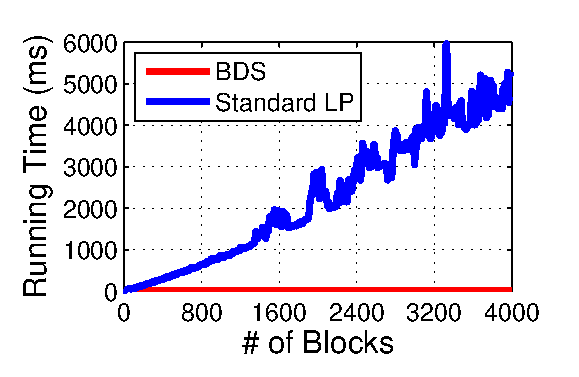
\includegraphics[width=\textwidth]{images/BDSvsLP.eps} % BDSvsLP.m
                \caption{The reduction on algorithm running time of \name over standard LP.}
                \label{fig:further:BDSvsLP}
        \end{subfigure}
	\hspace{0.1cm}
        \begin{subfigure}[b]{0.23\textwidth}
                \centering
                \includegraphics[width=\textwidth]{images/overlay.eps}
                \caption{The proportion of blocks downloaded from the original source.}
                \label{fig:further:overlay}
        \end{subfigure}
        \caption{[In-depth analysis] on (a) benefits of  approximations and (b) effects of overlay transmission.}
        \label{fig:further}
\vspace{-0.4cm}
\end{figure}

%\begin{figure}[t]
%  \centering
%  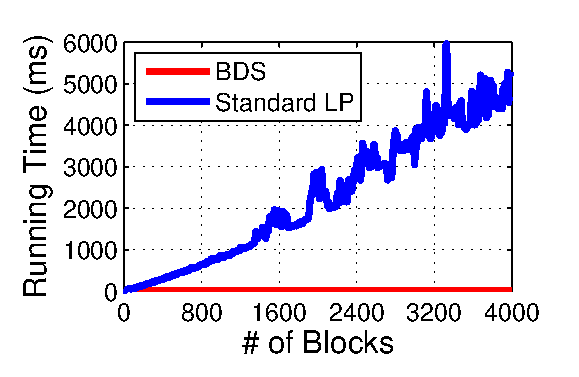
\includegraphics[width=45mm]{images/BDSvsLP.eps} % BDSvsLP.m
%  \caption{Algorithm running time of \name and standard LP.}
%  \label{fig:further:BDSvsLP}
%\end{figure}

\mypara{Optimization over algorithm running time} \name decouples scheduling and routing, which can significantly reduce the computational complexity. To clearly show the optimization, we measure the algorithm running time under \name and the standard linear programming (LP) solution. For the standard LP experiments, we use the \textit{linprog} library on MATLAB, set the upper bound of the iteration number ($10^6$) if the algorithm does not converge, and then record the CPU time various with block number. Figure \ref{fig:further:BDSvsLP} illustrates the comparison results, which shows that the running time of \name keeps under $25ms$ even with 3000 blocks (same as Figure \ref{fig:scale:cpu}) while that of standard LP grows quickly (nearly $4000ms$) with block number and will grow even higher with larger scale (we leave out that part in the figure).

%\begin{figure}[t]
%  \centering
%  \includegraphics[width=45mm]{images/overlay.eps}
%  \caption{The proportion of blocks downloaded from the original source.}
%  \label{fig:further:overlay}
%\end{figure}

\mypara{Availability of disjoint overlay paths} \Section\ref{subsec:motivation:case-for} reveals the observation that the benefits of application-level overlay networks depend critically on if there exist disjoint paths between two nodes. To explore the potential benefit, we record the ratio of the number of blocks downloaded from the original source to the total number of blocks, and the CDF is shown in Figure \ref{fig:further:overlay}. For about 90\% servers, the proportion of blocks downloaded from the original source is less than 20\%, which means that more than 80\% blocks are downloaded from other DCs on the disjoint paths, demonstrating great potential of multicast overlay network.

%\mypara{Breakdown of feedback loop delay} \name also applies the approximation of separating data scheduling from overlay routing, which can also reduce algorithm running time. We show the measurements on algorithm running time in Figure \ref{fig:analysis:time}. At the very beginning, the running time is nearly $800ms$, but drops to $300ms$ and even less quickly. This is because the separated scheduling stage selects only a subset of blocks, making the number of blocks decrease significantly and simplifying the routing decision making process.


%\begin{figure*}[t]
%        \centering
%        \begin{subfigure}[b]{0.3\textwidth}
%                \centering
%                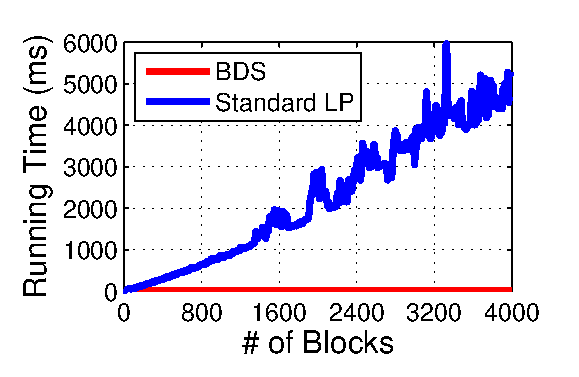
\includegraphics[width=50mm]{images/BDSvsLP.eps} % BDSvsLP.m
%                \caption{Algorithm running time of \name and standard LP.}
%                \label{fig:further:BDSvsLP}
%        \end{subfigure}
%        \begin{subfigure}[b]{0.3\textwidth}
%                \centering
%                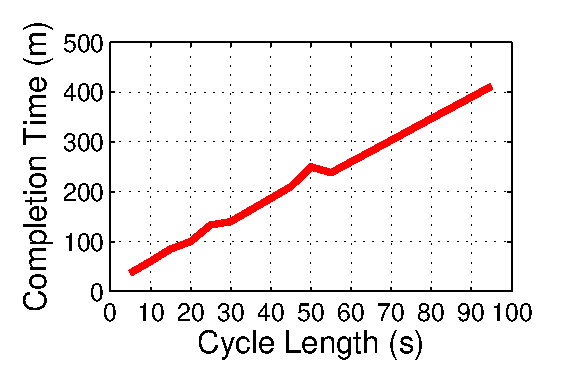
\includegraphics[width=50mm]{images/cycleDiff.eps}%cycleDiff.m
%                \caption{Completion time under different cycle lengths.}
%                \label{fig:further:cycleDiff}
%        \end{subfigure}
%        \begin{subfigure}[b]{0.3\textwidth}
%                \centering
%                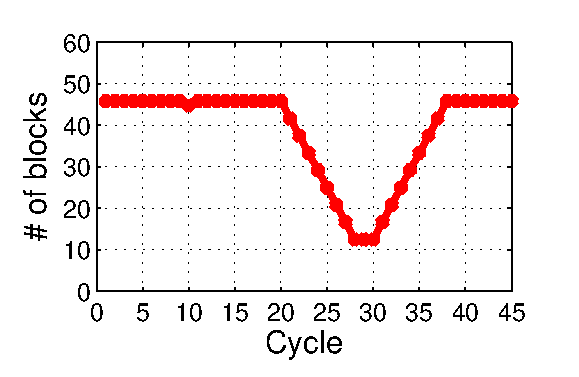
\includegraphics[width=50mm]{images/failure.eps}%fail.m
%                \caption{Average number of downloaded blocks per cycle under failures.}
%                \label{fig:further:failure}
%        \end{subfigure}
%        \caption{Further analysis on (1) running time, (2) cycle length, and (3) fault tolerance.}
%        \label{fig:further}
%\vspace{-0.4cm}
%\end{figure*}



In summary, both the prototype pilot deployed on \company network and the trace-driven simulations of \name achieve 3-5$\times$ speedup over existing solutions, with good scalability, fast algorithm convergence and lightweight resource consumption.


%\begin{itemize}
%\item Scalability of centralized control:
%\begin{itemize}
%\item Y: Bandwidth consumption, vs. X: \# of objects
%\item Y: Controller CPU usage, vs. X: \# of objects
%\item Y: Update delay vs. X: \# of objects
%\item Bar-chart to decompose update delay into collecting updates, running algorithm, and updating local agents
%\end{itemize}
%
%\item In-depth analysis:
%\begin{itemize}
%\item A graph to show the tradeoff caused by different update cycles (why 3 seconds is a good tradeoff?)
%\item Reduction on algorithm running time due to the approximation algorithm.
%\item Maybe another graph from the current 6.3?
%\end{itemize}
%
%\item Fault tolerance:
%\begin{itemize}
%\item Y: flow completion time, vs. X: time. Create a toy topology to send objects. The experiment begins with no failure. At time t1, one server is not available, and the graph should show Y only has performance degradation for less than 3 seconds; At time t2, the controller is not available, and the local agent should automatically revert to decentralized local control.
%\end{itemize}
%
%\end{itemize}




